%-------------------------------------------------------------------------------
%							PREAMBULE
%-------------------------------------------------------------------------------

\documentclass[notes]{beamer}
% \documentclass[notes,handout,aspectratio=169]{beamer}   % Use this to print notes and disable animations

%%----------Color and design section ---------------------------

%%% Define colors and main theme-----


\useoutertheme{infolines}

% \usecolortheme{spruce}
% \useinnertheme{circles}

% \useoutertheme{shadow}

% \usetheme{JuanLesPins}
\usetheme{Antibes}
% \usetheme{Bergen}

\useoutertheme{smoothbars}
\colorlet{mygreen}{green!50!blue} 
\definecolor{navy}{rgb}{0.04706, 0.13725, 0.26667}

% \usecolortheme{whale}
\usecolortheme[named=navy]{structure}


% \useinnertheme[shadow]{rounded}
\setbeamertemplate{itemize items}{$\blacktriangleright$}  %% Triangles in itmize

\setbeamercolor{alerted text}{fg=violet}
\setbeamercolor{alerted text}{fg=red!90!black}


% \setbeamertemplate{enumerate items}[default]

\setbeamertemplate{navigation symbols}{}
%%----------------------------------------------------------------

\usepackage[fontsize=8]{scrextend} % Use this to force the fontsize

\usepackage{docmute} % To include multiple files

\usepackage{ragged2e}   %% For justification
\usepackage{etoolbox}
\usepackage{listings}

\usepackage{xcolor}
\usepackage{graphicx}
% \sethlcolor{mDarkTeal}
\graphicspath{ {./img/} }



%\usepackage{amsmath,bm,mathtools}
\usepackage{amsmath,mathtools}
% \usepackage[mathrm=sym]{unicode-math}
% \usepackage{bigints}
% \setmathfont{Fira Math Regular} 
% \setsansfont[BoldFont={Fira Sans SemiBold}]{Fira Sans Regular}

\usepackage[utf8]{inputenc}
\usepackage[T1]{fontenc}
\usepackage{textcomp}
\usepackage[sansmath]{libertinust1math}
% \usepackage{eulervm}

% \usepackage[font=small,textfont=it,justification=centering]{caption}
\usepackage[font={bf},justification=centering]{caption}
\usepackage{subcaption}
% \captionsetup{labelformat=empty,labelsep=none}    % Pour retirer le terme figure des titres
% \setbeamerfont{caption}{family=\sffamily,size=\small}

\usepackage{marvosym} %% For smileys

\usepackage{multirow}

\usepackage{cases} 
\usepackage{siunitx}

\usepackage{mathdots}

\usepackage[backend=bibtex,style=authoryear,maxnames=2,natbib=true]{biblatex} % Use the bibtex backend with the authoryear citation style (which resembles APA)
\addbibresource{bibliography.bib} % The filename of the bibliography
\usepackage[autostyle=true]{csquotes} % Required to generate language-dependent quotes in the bibliography 
\renewcommand*{\bibfont}{\scriptsize} % Pour reduire la taille des references

\usepackage{hyperref}     %% No coloring for hyperlinks, since links are everywhere
\usepackage{booktabs}

\usepackage{xparse}   %% To define new commands


\usepackage{cancel}   %% TO strikeout text


\usepackage[british]{babel}
\usepackage[useregional]{datetime2}

%-------------------------------------------------------------------------------
%							NEW COMMANDS
%-------------------------------------------------------------------------------


\newcommand{\tabhead}[1]{{\bfseries#1}}

%\newcommand{\bvec}[1]{\bm{\mathrm{#1}}}  %% Use this to make vectors
\newcommand{\bvec}[1]{\symbfup{#1}}  %% Use this to make vectors
%\newcommand{\bmat}[1]{\bm{\mathsf{#1}}}   %% Use this to make tensors/

\newcommand{\myvec}[2]{\begin{pmatrix} #1  \\ #2 \end{pmatrix}}   %% vecteur 2d
\newcommand{\mymat}[4]{\begin{pmatrix} #1 & #2 \\ #3 & #4 \end{pmatrix}}  %% Matrice 2*2

\apptocmd{\frame}{}{\justifying}{} % Allow optional arguments after frame.
% \addtobeamertemplate{block begin}{}{\justifying}  %new code

\newcommand{\zerodisplayskips}{%        %% To remove space after math box
  \setlength{\abovedisplayskip}{0pt}%
  \setlength{\belowdisplayskip}{0pt}%
  \setlength{\abovedisplayshortskip}{0pt}%
  \setlength{\belowdisplayshortskip}{0pt}}
% \appto{\normalsize}{\zerodisplayskips}
% \appto{\small}{\zerodisplayskips}
% \appto{\footnotesize}{\zerodisplayskips}

% \cols                                       %% Easy way to create columns with justifiable content
\newcommand{\mycols}[1]{%
  \begin{columns}[onlytextwidth]
    #1
  \end{columns}
}
% % % \col{size}{title}{content}                  %% Easy way to create columns with optional titles
\newcommand{\mycol}[2]{%
    \column{.#1\textwidth-.25cm}{%
        \parbox[t]{\columnwidth}{%
        #2}%
    }%
}


\newcommand{\myfig}[2]{
  \begin{figure}       
    \frame{\includegraphics[width=\textwidth]{#1}}       
    \caption*{\textcolor{green}{Figure:} #2.}
  \end{figure}
}


\newcommand{\mycap}[1]{\caption*{\textcolor{green}{Figure:} #1.}}
\newcommand{\mycaptab}[1]{\caption*{\textcolor{green}{Table:} #1.}}


%-------------------------------------------------------------------------------
%							TITLE PAGE
%-------------------------------------------------------------------------------
\begin{document}

% \setbeamercolor{postit}{fg=white,bg=mDarkTeal}

\title[Deep learning for inverse problems in radiative transfer]{Simulation of light propagation and reconstruction of a medium's density using deep neural networks}

% \institute[University of Strasbourg]{\small \textbf{ \hspace*{0.1mm} Referent teacher} \hspace*{11mm} \textbf{Supervisors} \\ \footnotesize Christophe PRUD'HOMME \hspace*{4mm} Michel DUPREZ \\ \hspace*{38mm} Stephane COTIN}
\institute[]{\small Sorbonne Université}


\author[Roussel Desmond Nzoyem]{\large \bfseries Roussel Desmond Nzoyem}

% \logo{\includegraphics[width=0.6cm,height=1cm,keepaspectratio]{LogoBristol.png}}

\date[Soutenance mi-stage 2021]{\today}
% \date[Soutenance mi-stage]{\DTMdisplaydate{2021}{4}{20}{-1}}


\maketitle


%-------------------------------------------------------------------------------
%							INCLUDE THE CHAPTERS
%-------------------------------------------------------------------------------


\begin{frame}
  \small
  \frametitle{Contents}
  \tableofcontents
\end{frame}



%-------------------------------------------------------------------------------
%							FIRST SECTION
%-------------------------------------------------------------------------------

\section{\textsc{Motivation}}




\begin{frame}[fragile,t]
  \small
  \frametitle{Motivation}
  
  \note{
    \begin{description}
      \item Floe: Un floe est un morceau de glace;
      \item Albédo: la cryosphère reflette entre 90 et 95 \% des rayonnement recus par la planète.
    \end{description} 
  }

  \vspace*{-0.4cm}
  \begin{columns}[onlytextwidth,t]

    \mycol{50}{
      \begin{exampleblock}{Enjeux écologiques}
        \begin{itemize}
          \item Rôle crucial de la zone polaire pour le climat face au réchauffement climatique (SASIP)
          \item Prévisions climatiques à échelle nature
        \end{itemize}
      \end{exampleblock}

      \vspace*{-0.1cm}
      % \myfig{Ecological.jpg}{Image satellite de l'Arctique (MIZ Program, 2013)}
      \myfig{Ecological.png}{Évolution du gel saisonnier de l'Arctique \parencite{nasa2016arctic}}
      }

    \pause

    \mycol{50}{
      \begin{alertblock}{Enjeux industriels}
        \begin{itemize}
          \item Ouverture des routes maritimes pour l'exploitation des hydrocarbures
          \item Étude de l'interaction stations offshores / glace 
        \end{itemize}
      \end{alertblock}

      \vspace*{-0.1cm}
      \myfig{IceRoutesSlides.png}{Un bateau industriel dans la MIZ (O Globo, 2012)}

      }

    \end{columns}

    \note{La MIZ c'est la Maginal Ice Zone c'est cette zone où la glace est disloquée avec environ 80 per cent. C'est une zone idéale pour appliquer un modèle granulaire (les grains étant les floes, ou les morceaux de glace).
    Pendant que tu parle de l'interaction offshore/glace, il faut se poser la question de savoir qu'est ce cède des deux (ca va introduire mes objectifs)}

    \pause
    \normalsize
    \vspace*{-0.3cm}
    \begin{tcolorbox}[colback=red!40,colframe=red!30!black,arc=0mm,boxrule=0.2mm]
      \centering
      Il est donc urgent de prédire l’évolution de la banquise et de la MIZ (au moins) à court terme!
    \end{tcolorbox}
\end{frame}


% \section{\textsc{Introduction2}}
\setbeamercovered{transparent}

\begin{frame}{Objectifs}

  \begin{exampleblock}{Objectifs généraux}

    \begin{itemize}
      \item Comprendre le modèle de rupture de Griffith; \pause
      \item Comprendre le passage micro/macro de la percussion; \pause 
      \item Intégrer le modèle dans un code de calcul à l’échelle des floes de glace.
    \end{itemize}
  \end{exampleblock}

  \setbeamercovered{invisible}
  \pause

  \begin{block}{Objectifs intermédiaires}

    \begin{enumerate}
      \item Prise en main de la notion de $\Gamma$‑convergence;
      \item Lecture des travaux précédents:
      \begin{itemize}
        \item \alert{M. Rabatel, S. Labbé, et J. Weiss}: Dynamics of an assembly of rigid ice floes (\citeyear{rabatel2015dynamics}); 
        \item \alert{Matthias Rabatel}: Modélisation dynamique d’un assemblage de floes rigides (\citeyear{rabatel2015modelisation});
        \item \alert{Dimitri Balasoiu}: Modélisation et simulation du comportement mécanique de floes de glace (\citeyear{balasoiu2020modelisation}).
      \end{itemize}
      
      \item Modélisation et simulation du déplacement des n\oe{}uds d'un floe isolé:
      \begin{itemize}
        \item en 1D;
        \item en 2D;
      \end{itemize}

      \item Introduction de la percussion et de la fracture dans le code préexistant.

    \end{enumerate}
  \end{block}

\end{frame}

\setbeamercovered{invisible}

% 
%-------------------------------------------------------------------------------
%							SECOND SECTION
%-------------------------------------------------------------------------------

\section{\textsc{État de l'art}}


\subsection{Thèse de M. Rabatel}


\begin{frame}{Cinétique du floe}
  \mycols{
    \mycol{50}{
      Les équations de Newton-Euler:
      \begin{align} \label{eq:neweu}
      \begin{dcases} 
        M_i \frac{\diff \dot{\bvec{G}}_i(t)}{\diff t} &= \bvec{F}_i, \\
        \mathcal{I}_i \frac{\diff \dot{\theta}_i(t)}{\diff t} &= \mathfrak{M}_i,
      \end{dcases}        
      \end{align}
      où pour le floe $\Omega_i$ : 
      \begin{itemize}
        \item $M_i$ : masse du floe;
        \item $\bvec{F}_i$ : somme des forces par unité de volume;
        \item $\mathcal{I}_i$ : moment d'inertie;
        \item $\mathfrak{M}_i$ : moment dynamique en $G$.
      \end{itemize}
      Le système (\ref{eq:neweu}) se réécrit sous la forme :
      \begingroup
      \color{red}
      \begin{align*}    
          \mathcal{M}_i \frac{\diff W_i(t)}{\diff t} = \mathcal{H}_i(t) ,
      \end{align*}
      \endgroup
      avec 
      \begin{align*}
      \mathcal{M}_i = 
      \begin{pmatrix}
          M_i & 0 & 0 \\ 0 & M_i & 0 \\ 0 & 0 & \mathcal{I}_i
      \end{pmatrix} , \quad
      W_i(t) = 
      \begin{pmatrix}
          \dot{\bvec{G}}(t) \\ \dot{\theta}_i(t)
      \end{pmatrix} , 
      \text{ et } \quad \mathcal{H}_i(t) = 
      \begin{pmatrix}
          \bvec{F}_i(t) \\ \mathfrak{M}_i(t)
      \end{pmatrix}.
      \end{align*}
    }


    \mycol{50}{
      \myfig{FloeRabatel}{Repères abosolu et local pour un floe \parencite{rabatel2015modelisation}}
    }
  }
  
\end{frame}



\begin{frame}{Interaction entre les floes}
  \mycols{

    \mycol{45}{
      \myfig{Collision1.png}{Interaction entre deux floes $\Omega_k$ et $\Omega_l$ au point $P_j$ \parencite{rabatel2015modelisation}}
    }

    \mycol{55}{Deux conditions à respecter:
    \begin{enumerate}
      \item \textbf{Condition unilatérale de Signorini} : afin de décrire la condition de non-interpénétration:
      \begin{tcolorbox}[colback=myblack2!5,colframe=myblack2!30!black,arc=0mm,boxrule=0.1mm]
        \textit{\footnotesize S’il y a contact, alors la réaction est strictement positive et l’accélération relative nulle, et s’il n’y a pas contact, alors l’accélération relative est strictement positive et la réaction nulle.}
      \end{tcolorbox}
      \normalsize
      \pause
      \item \textbf{Loi de friction de Coulomb} : afin de modéliser le comportement de friction pendant une collision:
      \begin{tcolorbox}[colback=myblack2!5,colframe=myblack2!30!black,arc=0mm,boxrule=0.1mm]
        \textit{\textit{\footnotesize Pendant la collision, y a-t-il frottement statique, ou y a-t-il glissement (suivant la direction $\bvec{T}_j$ ou $-\bvec{T}_j$)}?}
      \end{tcolorbox}
      \normalsize
    \end{enumerate}}

    \note{Historiquement, on distingue ici deux approches:
    \begin{itemize}
      \item l'approche par régularisation: Hertz (force de contact proportionnelle à la distance d'inter-penetration); largement répandues en robotique, en VR, habits, etc...MAIS ON NE VEUT PAS D'INTERPÉNÉTRATION !
      \item l'approche non-régulière: développée par inclusion différentielle: efficace, mais difficile à manipuler. D'ou l'essort des méthodes LCP. 
    \end{itemize}}

  }

\end{frame}



\begin{frame}{Discussion sur la thèse}

  \mycols{

    \mycol{37}{
      \begin{itemize}
        \item Les floes sont rigides;
        \item Le modèle ne gère pas la rhéologie de la glace;
        \item Les coefficients de friction et de restitution sont limitants.
      \end{itemize}
    }

    \mycol{27}{
      \myfig{Derive.png}{Configuration initiale \parencite{rabatel2015modelisation}}
    }

    \mycol{32}{
      \begin{figure}[!h]
        \begin{subfigure}[b]{0.60\textwidth}
            \centering
            \includegraphics[width=\textwidth]{DeriveBlock2.png}
            \caption{à 2h04}
        \end{subfigure}
        \begin{subfigure}[b]{0.60\textwidth}
            \centering
            \includegraphics[width=\textwidth]{DeriveBlock3.png}
            \caption{à 3h40}
          \end{subfigure}
           \caption{Dérive sous l'effet de la force de Coriolis \parencite{rabatel2015modelisation}}
    \end{figure}

    }

  }

\end{frame}




\subsection{Thèse de D. Balasoiu}


\begin{frame}{Un modèle de fracture variationnel (Francfort-Marigo)}
  L'énergie totale s'écrit :
  \begin{tcolorbox}[colback=myblack2!5,colframe=myblack2!30!black,arc=0mm,boxrule=0.1mm]
    \vspace{-0.4cm}
    \begin{align*}
      \etot : \,\bigcup_{\sigma \in \Sigma } A_{\sigma} \times \left\{ \sigma \right\} &\rightarrow \mathbb{R} \\
      u &\mapsto \textcolor{orange}{\int_{\Omega \backslash \sigma} Ae(u) : e(u) \diff x} + \textcolor{magenta}{k\mathcal{H}^1(\sigma)}.
    \end{align*}
    \vspace{-0.4cm}
  \end{tcolorbox}
  
  \pause
  Une solution du problème de fracture fragile est un couple $(u^*, \sigma^*)$ qui vérifie:
  \vspace*{0.25cm}
  $$
  \etot(u^*,\sigma^*) = \min_{\sigma \in \Sigma}{\min_{u\in A_{\sigma}}{\etot(u,\sigma)}} \,.
  $$

	\note{$\Sigma$ c'est l'ensemble des fractures admissibles, et $A_{\sigma}$ l'ensemble des déplacements admissibles sur un floe qui présente déjà la fissure $\sigma$.
  Ne pas oublier de préciser quel est exactement l'aproche de Griffith (compétition d'énergies). Et quel est l'approt de Francfort-Marigo (Formulation variationnelle). Et Bourdin (Regularisation)}

  \myfigsize{PhaseField2.png}{Bifurcation d’une fracture \parencite{nagaraja2019phase}}{90}

\end{frame}


\begin{frame}{Réseaux de ressorts à grande raideur}

  \myfigsize{Ressort2.png}{Réseau de ressorts régulier \parencite{balasoiu2020modelisation}}{20}

  \vspace*{-0.25cm}
  \myfigsize{VoronoiDelaunay.png}{Tirage de points et diagrammes de Voronoi (à gauche) et Delaunay (à droite) \parencite{balasoiu2020modelisation}}{60}

  \note{la première figure est un réseau de ressort dans Z. Balasoiu montre qu'il s'agit là d'une bonne approximation d'un matériau élastique à travers une résultat de Gamma convergence qu'il prouve, tout comme avec la deuxième figure. La deuxième figure fait suite à une tirage par Processus de Poisson (pourquoi Poisson?) pour obtenir le nombre de points. Les coordonnées sont obtenus par des lois uniforme. Et enfin on fait un diagramme de Voronoi, et puis un de Delaunay (pronunciation de Delaunay ?).}

  \note{  AFIN d'établir la condition de Dirichlet nécéssaire pour engendrer la fracture, on passe du modèle macroscopique à un modèle microscopique.}

\end{frame}


% 
%-------------------------------------------------------------------------------
%							THIRD SECTION
%-------------------------------------------------------------------------------



\section{\textsc{Results in 1D}}


\subsection{Simulation}


\begin{frame}[fragile]
  \frametitle{Example of a 1D simulation}

  \begin{center}
    \textcolor{violet}{\href{run:../img/Video1D.mp4}{Click here for the RTE simulation in 1D.}}
    % \href{run:./img/Video1D.mp4}{Click here for the RTE simulation in 1D.}
  \end{center}

% \begin{center}
%   \includemedia[
%     width=0.95\linewidth,
%     activate=pageopen,
%     addresource=Video1D.mp4,
%     flashvars={
%        source=Video1D.mp4
%       &autoPlay=true
%     },
%     passcontext, % enable VPlayer's right-click menue
%   ]{\includegraphics{Thumbnail1D.png}}{VPlayer.swf}%
% \end{center}

\end{frame}

\begin{frame}[fragile]
  \frametitle{Inputs/outputs in 1D}

  \begin{block}{\vspace*{-3cm}}
    \centering The data gathered from the simulations is post-processed (resampled, normalized, etc.). 
  \end{block}

  \begin{columns}
  \begin{column}{0.7\textwidth}
      \begin{figure}
      \includegraphics[width=8cm]{EntreeSortie1D}       
      \mycap{An input for the Neural Network (above) and the awaited output (below)}
      \end{figure}
   \end{column}
   \begin{column}{0.3\textwidth}
      \begin{figure}
      \includegraphics[width=3cm]{Entrees1D}       
      \mycap{Size of an input (from the right boundary)}
      \end{figure}
      \begin{figure}
        \includegraphics[width=2cm]{Sortie1D.png}       
        \mycap{Size of an output}
      \end{figure}
   \end{column}
  \end{columns}

\end{frame}




\subsection{Model, training, and predictions}



\begin{frame}
  \frametitle{The architecture in Keras}
  \begin{center}
      %%% Ajouter l'image des hierarchie de machine learning
      \begin{figure}
      \includegraphics[width=.95\textwidth]{DRNNNew.png}    % Modifier la sortie pour avoir 1D/Class2D/Reg 2D
      \mycap{CNN used for the 1D inverse problem}
      \end{figure}
  \end{center}
\end{frame}



\begin{frame}
  \frametitle{Hyper-parameters and training}

  \begin{table}[h!]
      \scriptsize
      \label{tab:Parametres}
      \centering
      \begin{tabular}{l l}
      \toprule
      \textbf{Hyper-parameter} & \hspace*{2mm}\textbf{Value} \\
      \midrule
      % \onslide<+>
      optimizer  & Adam \\
      learning rate  & 1e-4, 1e-5, etc. \\
      batch size  & 32 \\
      epochs  & 100 \\
      patience  & 10 \\
      kernel size  & 3 \\
      activation  & relu, linear, sigmoid \\
      \bottomrule
      \end{tabular}
      \mycaptab{List of the most important hyper-parameters for the training}
  \end{table}

  \myfig[7][train1D]{CourbeTraining1D.png}{$MSE$ loss and $R^2$ accuracy during training and validation}

\end{frame}


\begin{frame}[fragile]
  \frametitle{Best/worst predictions}

  \begin{columns}
  \begin{column}{0.5\textwidth}
      \begin{figure}
      \includegraphics<1->[width=4cm]{Meilleur1D2}       
      \includegraphics<1->[width=4cm]{Meilleur1D1}       
      \only<1->{\mycap{The 2 best predictions}}
      \end{figure}
   \end{column}
   \begin{column}{0.5\textwidth}
      \begin{figure}
      \includegraphics[width=4cm]{Pire1D1}       
      \includegraphics[width=4cm]{Pire1D2}       
      \only{\mycap{The 2 worst predictions}}
      \end{figure}
   \end{column}
  \end{columns}

\end{frame}


\begin{frame}
  \frametitle{The obtained scores}

  \begin{table}[h!] 
      \centering
      \begin{tabular}{l l}
      \toprule
      \textbf{Score name} & \textbf{Value} \\
      \midrule
      $R^2$ & 45.50 \%\\
      \textbf{Personalized} & 28.21 \%\\
      \bottomrule
      \end{tabular}
      \mycaptab{Prediction results on the Test dataset in 1D}
  \end{table}

  \begin{columns}
       \begin{column}{0.5\textwidth}
          \begin{figure}
          \includegraphics<1>[width=3cm]{Hauteur1D}       
          \only<1>{\mycap{Correlation between observed and predicted \alert{heights} of the obstacles}}
          \end{figure}
       \end{column}
       \begin{column}{0.5\textwidth}
        \begin{figure}
        \includegraphics<1->[width=3cm]{Position1D}       
        \only<1->{\mycap{Correlation between observed and predicted \alert{positions} of the obstacles}}
        \end{figure}
     \end{column}
  \end{columns}

\end{frame}


\metroset{background=dark}

\begin{frame}
  \frametitle{Conclusion on the 1D inverse problem}
  
  \begin{alertblock}{\textbf{What we found out in 1D is:}}
    \begin{enumerate}
      \item We are able to determine the size of the tumours (obstacles);
      \item However, we cannot locate them.
    \end{enumerate}
    The 1D inverse problem appears to be ill-posed. We could try solving the issue by increasing the dimensionality.
  \end{alertblock}
\end{frame}

\metroset{background=light}




% 
%-------------------------------------------------------------------------------
%							FOURTH SECTION
%-------------------------------------------------------------------------------


\section{\textsc{Travaux 2D}}


\subsection{Déplacement des n\oe{}uds}


\begin{frame}{Déplacement des n\oe{}uds d'un floe isolé (1)}

    \mycols{

        \mycol{40}{

            \begin{figure}
                \centering
                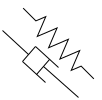
\includegraphics[width=0.6\textwidth]{Deplacement2D-1.png}
                \caption{Floe de glace 2D \vspace{0.5cm}}
            \end{figure}

        }

        \mycol{60}{
            % \onslide<2>{\myfig{PlotDeplacement2D-1-NonConv.png}{Simulation avec $T=10$}}

            \begin{figure}
                \centering
                \includegraphics<2>[width=\textwidth]{PlotDeplacement2D-1-NonConv.png}
                \onslide<2>{\caption{Simulation avec $T=10$} \vspace{-0.5cm}}
            \end{figure}
            % \myfig{PositionInitFinales.png}{Illustration à $T=4$}
        }

    }

	% \onslide<1>{\vspace{0.5cm}}

	% \onslide<2>{\vspace{-1cm}}
    Les équations de Newton-Euler :
    \begin{align*}
        \forall i \in \mathbb{Z}/3\mathbb{Z}, \quad m \ddot{\bvec{q}}_i = \underbrace{\sum_{j=i+1}^{i+2} \textcolor{teal}{C_{ij}} \left[  \textcolor{blue}{k \left( \Vert \bvec{q}_j - \bvec{q}_i \Vert - L_{ij} \right) \bvec{u}_{ij}} \textcolor{orange}{- \mu \left\langle \dot{\bvec{q}}_j - \dot{\bvec{q}}_i, \, \bvec{u}_{ij}  \right\rangle  \bvec{u}_{ij}}  \right]}_{\bvec F_i} . 
    \end{align*}

    \vspace{-0.2cm}
    Schéma d’Euler explicite :
    \begin{align*}
        \bvec{q}_{i}^{n+1} = 2\bvec{q}_{i}^{n}-\bvec{q}_{i}^{n-1} + \frac{\Delta t^2}{m} \sum_{j=i+1}^{i+2}C_{ij}\left[ k \left( \Vert \bvec{q}_j^n - \bvec{q}_i^n \Vert - L_{ij} \right) \bvec{u}_{ij} - \frac{\mu}{\Delta t} \left\langle \bvec{q}_{j}^{n}-\bvec{q}_{j}^{n-1} - \bvec{q}_{i}^{n}+\bvec{q}_{i}^{n-1}, \, \bvec{u}_{ij} \right\rangle  \bvec{u}_{ij}  \right].
    \end{align*}
    
\end{frame}


\begin{frame}[fragile]{Déplacement des n\oe{}uds d'un floe isolé (2)}

    \tiny
    \begin{lstlisting}[language=Python,caption=Code de simulation et schéma avec Scipy]
                                    q0 = np.stack([q1_0, dotq1_0, q2_0, dotq2_0, q3_0, dotq3_0])
                                    q0_ = np.reshape(q0, (nb_nodes*4))

                                    def model(t, Q_):
                                        Q = np.reshape(Q_, (nb_nodes*2, 2))
                                        Q_ret = np.zeros_like(Q)
                                        Q_ret[2*0] = 0; Q_ret[2*1] = 0
                                        
                                        for i in range(1, nb_nodes):  ## <-- Node 0 is immobilized
                                            Q_ret[2*i] = Q[2*i+1] 
                                            
                                            for neighbor in range(i+1, i+3):
                                                j = neighbor % nb_nodes
                                                u[i,j] = (Q[2*j] - Q[2*i]) / nplin.norm(Q[2*j] - Q[2*i])
                                                Q_ret[2*i+1] += (1 / m)*C[i,j]*( k*(nplin.norm(Q[2*j]-Q[2*i]) - L[i,j])*u[i,j]
                                                                -  mu*(np.dot(Q[2*j+1] - Q[2*i+1], u[i,j]))*u[i,j] )
                                        return np.reshape(Q_ret, (nb_nodes*4))

                                    sol = solve_ivp(model, [0,T], q0_, t_eval=t)
    \end{lstlisting}
    
	\hspace*{-1cm}
	\mycols{
	
	\mycol{70}{
	    \begin{figure}
        \centering
        \hspace{-1cm}
        \includegraphics[width=0.8\textwidth]{PositionInitFinales.png}
        %\hspace{-1.5cm}
        \caption{Illustration à $t=0$ et $t=4$}
    	\end{figure}
	}
	
	\hspace{-0.5cm}
	
	
	\mycol{32}{

	% \vspace{-0.5cm}
	% \normalsize
	% \hspace{-1cm}
	% \begin{adjustwidth}{1cm}{2cm}
	%    \begin{alertblock}{En somme}
    %      Avec un schéma Euler explicite, symplectique ou Scipy (RK45), il faut fixer certains n\oe{}uds pour que le système reste stable!
    %     \end{alertblock}
	% \end{adjustwidth}	

    \scriptsize
    \begin{tcolorbox}[colback=red!5,colframe=red!50!black,arc=0mm,boxrule=0.1mm,title=Observation]
        \vspace*{-0.1cm}
            Avec un schéma Euler explicite, symplectique ou Scipy (RK45), il faut fixer certains n\oe{}uds pour que le système reste stable!
        \vspace*{-0.1cm}
    \end{tcolorbox}

	}	
	\normalsize
	}
	

\end{frame}




\subsection{Percussion entre floes}


\begin{frame}{Collision parfaitement inélastique entre deux floes (1)}

    \mycols{

        \mycol{40}{
			\myfigframe{Percussion2DNew.png}{Illustration de la percussion 2D}

\begin{align*}
\begin{dcases}
    (m+m') \ddot{\bvec{q}}_0  = \bvec{F}_0 + \bvec{F}^{'}_0  , & \textcolor{cyan}{\text{(SE)}} \\
    \ddot{\bvec{p}}_0 = \ddot{\bvec{q}}_0 , \dot{\bvec{p}}_0 = \dot{\bvec{q}}_0 , \bvec{p}_0 = \bvec{q}_0 - \Delta_0 , & \textcolor{cyan}{\text{(SE)}} \\
    m \ddot{\bvec{q}}_i = \bvec{F}_i   \,, \quad \quad \quad \forall 1 \leq i \leq n-1 , & \textcolor{orange}{\text{(SI)}} \\
    m' \ddot{\bvec{p}}_i = \bvec{F}^{'}_i   \,, \quad \quad \quad \forall 1 \leq i \leq n'-1 , & \textcolor{orange}{\text{(SI)}}
\end{dcases}
\end{align*}
où : $\quad \Delta_0 = \bvec{q}_0(0) - \bvec{p}_0(0)$.
			
        }

        \pause
        \mycol{60}{
            \myfigframesize{Percussion2DSlides}{Un maillage 2D par processus de Poisson}{80}
            
            \centering
            \textcolor{mygray}{\href{run:../../../../Share/ShortAnim2D.gif}{\textbf{Animation de la percussion 2D}}}

            \only<2>{
            \animategraphics[loop,controls,autoplay,width=0.9\linewidth]{10}{Simu2D/ShortAnim2D-}{0}{70}
            }

        }

    }
    
\end{frame}




\begin{frame}{Collision parfaitement inélastique entre deux floes (2)}

	\myfigframesize{ClientWebMoi.jpg}{Client web développé et maintenu avec \textcolor{red}{Flask}}{60}
	\note{En fin je dois vous montrer ce clien web.  Je ne pouvais m'en empécher.}
    
\end{frame}


% 
%-------------------------------------------------------------------------------
%							FITH SECTION
%-------------------------------------------------------------------------------

\section{\textsc{Conclusion}}


\subsection{Bilan}

\setbeamercovered{transparent}
\begin{frame}{Apports et recherches ultérieures}

    \vspace{-0.2cm}
	\myfigsize{Timeline}{Résumé du déroulement du stage}{65}
	\note{Prendant la soutenance, et dans le rapport, il faut dire que j'ai utilisé une méthode Agile. Plus précisément Scrum. Même si cela n'était aps très formel, j'implémentais une fonctionnalité chaque semaine; sauf que pour le dernier mois de stage, il a fallut coder un gros truc.. }

	\note{On a commencer par la lecture des travaux antérieus, et on a fini par la percussion 1D en pasant par la percussion 2D. Ca semble contre-intuitif MAIS c'est nécésssaire pour avancer.}
	\pause
	\small
	
    \vspace{-0.3cm}
	\mycols{	
		
		\mycol{50}{
        \begin{alertblock}{Recherches ultérieures}
        \begin{itemize}
        \item Implémentation de la méthode du champ de phase;
        \item Implementation de la fracture au problème 2D, 2.5D, ou 3D;
        \item Intégration de la fracture au code de \citeauthor{rabatel2015modelisation};
        \item Confirmation de l'approximation par réseaux de ressorts;
        \item Optimiser les codes avec Cython ou en C++;
        \item Tests de validation en laboratoire.
        \end{itemize}
		\end{alertblock}
		}

        \pause
        \note{Pour le passage en dimension supérieure, mentionner le CoD Curse of Dimensionnalyty qui s'est posé lorsque je suis passé de la 1D à la 2D, et qui se passera en passant à la 3D}


		\mycol{50}{
        \begin{exampleblock}{Apports du stage}
        \begin{itemize}[<+->]
        \item Simulation de systèmes dynamiques en Python;
        \item Prise en main du modèle de rupture de Griffith (analyse fonctionnelle, analyse numérique, etc.);
        \item Maitrise de l'approche par réseaux de ressorts (probabilité, raisonnance);
        \item Utilisation de TikZ, Flask, Bokeh, Symbolab, et bien d'autres;
        \item Recherche en milieu professionnel;
        \item Savoir-faire transférables (vision globale, etc.).
        \end{itemize}
		\end{exampleblock}
		}
        
        \note{Blague sur TikZ: La loi de Murphy. Etant donné assez de temps, tout peut arriver. C'est comme ca j'ai apris TIKZ, en 6 mois !!}

		
	}
    
\end{frame}




\subsection{Délivrables}

\begin{frame}{Liste récapitulative et délivrables}

        \begin{block}{Checklist des objectifs}
    	\begin{enumerate}
      	\item[\checkmark] Prise en main de la notion de $\Gamma$‑convergence; \pause
      	\item[\checkmark] Assimilation des travaux antérieurs; \pause
      	\item[\checkmark] Modélisation de la percussion (1D et 2D); \pause
      	\item[\checkmark] Modélisation de la fracture: 
      	\begin{itemize}
        \item[\checkmark] en 1D;
        \item[$\times$] en 2D. 
        \end{itemize} \pause
      	\item[$\times$] Calculs à l'échelle des floes de glace de l'Arctique. 
      	\end{enumerate}
		\end{block}
	
        \setbeamercovered{invisible}
        \pause
        \begin{exampleblock}{Délivrables}
        \begin{enumerate}
        \item Rapport de stage: \myemoji \textcolor{orange}{\href{https://github.com/desmond-rn/ice-floes/tree/master/pdf}{ GitHub}};
        \item Code de calcul: \myemoji \textcolor{orange}{\href{https://github.com/desmond-rn/ice-floes/tree/master/code}{ GitHub}} et \myemoji \textcolor{orange}{\href{https://framagit.org/RaK/SimuRessorts}{ Framagit}};
        \item Quelques simulations: \myemoji \textcolor{orange}{\href{https://seafile.unistra.fr/d/a6c3680909624b22be7c/}{ Seafile}}.
        \end{enumerate}
		\end{exampleblock}
    
\end{frame}




% %-------------------------------------------------------------------------------
% %							THE BIBLIOGRAPHY
% %-------------------------------------------------------------------------------

\appendix   % Pour retirer les references de la bare de navigation
% \vspace*{0.5mm}


% \hspace*{-0.75cm}\parbox[t]{\textwidth} 

\tiny
\printbibliography

% %-------------------------------------------------------------------------------
% %							THANK YOU NOTE 
% %-------------------------------------------------------------------------------

  \begin{frame}
    \Large
    \begin{exampleblock}{\centering \LARGE Thank you for your kind attention \Large \Smiley{} !}\LARGE
      \centering
      Questions ?
    \end{exampleblock}

  \end{frame}


\end{document}

